% *********** Section 5 % *********** %

\section{Functionalities Implemented to satisfy requirements}
For each of the required entities we have implemented PHP functions to Create, Read, Update and Delete a resource. These functions are placed in our Ressource controllers which handle the requests coming from the front end to our API. To make our live's simpler we have implemented the following helper functions accessible by all the rest of our controllers.
\begin{minted}{php}
<?php
public function doInsertAndGetId($tableName, Collection $parameters){
        $keys = $parameters->keys()->join(',');
        $placeholders = $parameters->map(function () { return '?';})->join(',');
        $result = DB::insert("INSERT INTO $tableName (
                $keys
            ) VALUES ($placeholders)",
            [
                ...$parameters->values(),
            ]
        );
        if ($result) {
            $id = DB::getPdo()->lastInsertId();
            return $id;
        }
        return null;
    }
    
\end{minted}

\begin{minted}{php}
<?php
public function doUpdate($tableName, $key, $id, Collection $fieldsToUpdate){
        $values = $fieldsToUpdate->values();
        $values->push($id);
        return DB::update("UPDATE $tableName SET {$fieldsToUpdate->keys()->join(',')} WHERE $key = ?", $values->toArray());
    }
\end{minted}

\begin{minted}{php}
<?php
public function syncGroupIds($personId, $groupZones)
    {
        $toDelete = collect();
        $toAdd = collect();

        if (!$personId) {
            abort(500);
        }

        // delete anything that isn't in the group_zones
        $dbGroupIds = collect(DB::select("SELECT gzp.group_id FROM GroupZonePersonPivot gzp
	            WHERE person_id = '{$personId}'"))->pluck('group_id')->toArray();
        foreach ($dbGroupIds as $dbGroupId) {
            if (!in_array($dbGroupId, $groupZones)) {
                $toDelete->push($dbGroupId);
            }
        }
        foreach ($groupZones as $groupZone) {
            if (!in_array($groupZone, $dbGroupIds)) {
                $toAdd->push($groupZone);
            }
        }
        if ($toAdd->isNotEmpty()) {
            $stringAdd = $toAdd->map(function ($groupId) use (&$personId) {
                return "($personId,$groupId)";
            })->join(',');
            DB::insert("INSERT INTO GroupZonePersonPivot (`person_id`, `group_id`)
                VALUES $stringAdd");
        }
        if ($toDelete->isNotEmpty()) {
            $toDelete->map(function ($id) use (&$personId) {
                DB::insert("DELETE FROM GroupZonePersonPivot WHERE person_id=$personId and group_id=$id");
            });
        }
    }
\end{minted}
\subsection{Patient CRUD}
\subsubsection{Create}
\begin{minted}{php}
<?php
public function create(Request $request){
        $parameters = collect($request->only([
            'medicare',
            'first_name',
            'last_name',
            'address',
            'postal_code',
            'postal_code_id',
            'citizenship',
            'email',
            'phone',
            'dob'
        ]));
        $parameters['medicare'] = str_replace(' ', '' , $parameters['medicare']);
        $parameters->put('password', bcrypt(str_replace('-','',$parameters['dob'])));
        $parameters->put('api_token', Str::random(60));
        $id = $this->doInsertAndGetId('Person', $parameters);
        $this->syncGroupIds($id, $request->group_zones);
        DB::insert("INSERT INTO Patient (person_id) VALUES (?)", [$id]);
        return response()->json(['patient_id' => $id], $id ? Response::HTTP_CREATED : Response::HTTP_BAD_REQUEST);
}
    
\end{minted}
\subsubsection{Read}
\begin{minted}{php}
<?php
 public function readAll(Request $request){
        return response()->json(DB::select("SELECT p.patient_id, ps.*
            FROM Patient p
            JOIN Person ps ON p.person_id = ps.person_id"));
}

 public function readOne($id){
        $result = DB::select("SELECT
                p.patient_id,
                ps.*,
                c.city,
                pv.province,
                r.region_name,
                GROUP_CONCAT(gzp.group_id) as 'group_zones'
            FROM Patient p
            JOIN Person ps ON p.person_id = ps.person_id
            LEFT JOIN GroupZonePersonPivot gzp ON gzp.person_id = p.person_id
            JOIN PostalCode pc ON ps.postal_code_id = pc.postal_code_id
            JOIN City c ON pc.city_id = c.city_id
            JOIN Region r ON c.region_id = r.region_id
            JOIN Province pv ON pv.province_code = r.province_code
            WHERE p.patient_id = '{$id}'
            GROUP BY p.patient_id");

        return response()->json((count($result) > 0 ? $result[0] : null),
            count($result) > 0 ? 200 : 404
        );
}

\end{minted}

\subsubsection{Update}
\begin{minted}{php}
<?php
 public function update(Request $request, $id){
        $personFieldsToUpdate = collect();

        if ($request->filled('password')) {
            $personFieldsToUpdate->put('password = ?', $request->password);
        }
        if ($request->filled('first_name')) {
            $personFieldsToUpdate->put('first_name = ?', $request->first_name);
        }
        if ($request->filled('last_name')) {
            $personFieldsToUpdate->put('last_name = ?', $request->last_name);
        }
        if ($request->filled('address')) {
            $personFieldsToUpdate->put('address = ?', $request->address);
        }
        if ($request->filled('postal_code_id')) {
            $personFieldsToUpdate->put('postal_code_id = ?', $request->postal_code_id);
        }
        if ($request->filled('citizenship')) {
            $personFieldsToUpdate->put('email = ?', $request->email);
        }
        if ($request->filled('email')) {
            $personFieldsToUpdate->put('phone = ?', $request->phone);
        }
        if ($request->filled('phone')) {
            $personFieldsToUpdate->put('phone = ?', $request->phone);
        }
        if ($request->filled('dob')) {
            $personFieldsToUpdate->put('dob = ?', $request->dob);
        }
        $personId = DB::select("SELECT person_id FROM Patient WHERE patient_id = '{$id}'")[0]->person_id ?? null;
        if (!$personId) {
            abort(500);
        }
        $this->syncGroupIds($personId, $request->group_zones);
        $this->doUpdate('Person', 'person_id', $id, $personFieldsToUpdate);
        $fieldsUpdated = $personFieldsToUpdate->count();
        return response()->json(['message' => $fieldsUpdated . " field(s) updated successfully!"], 200);
}

\end{minted}
\subsubsection{Delete}
\begin{minted}{php}
<?php
public function delete($id){
        $status = DB::delete("DELETE FROM Patient WHERE patient_id = ?", [$id]);
        return response()->json(['status' => "Deleted successfully!"], 200);
}

\end{minted}

\subsection{Public Health Worker CRUD}
\subsubsection{Create}
\begin{minted}{php}
<?php
public function create(Request $request){
        $parameters = collect($request->only([
            'medicare',
            'password',
            'first_name',
            'last_name',
            'address',
            'postal_code_id',
            'citizenship',
            'email',
            'phone',
            'dob',
            'region_id'
        ]));
        $pid = $this->doInsertAndGetId('Person', $parameters);

        $this->syncGroupIds($pid, $request->group_zones);
        $schedule = $request->input('schedule');
        $position_id = $request->input('position_id');
        $center_id = $request->input('health_center_id');

        DB::insert("INSERT INTO PublicHealthWorker (person_id, position_id, schedule, health_center_id) VALUES (?,?,?,?)", [$pid, $position_id, $schedule, $center_id]);
    }
\end{minted}
\subsubsection{Read}
\begin{minted}{php}
<?php
 public function readAll(Request $request){
        $stringSearch = "SELECT w.health_worker_id, pst.position, w.schedule, ps.*
            FROM PublicHealthWorker w
            JOIN Position pst ON w.position_id = pst.position_id
            JOIN Person ps ON w.person_id = ps.person_id
            JOIN PublicHealthCenter phc ON w.health_center_id = phc.health_center_id";

        if ($request->filled("health_center_id")) {
            $stringSearch .= " WHERE w.health_center_id = " . $request->health_center_id;
        }
        return response()->json(DB::select($stringSearch));
}
    public function readOne($id){
        $result = DB::select("SELECT
                w.health_worker_id,
                pst.position,
                w.schedule,
                ps.*,
                c.city,
                p.province,
                r.region_name,
                GROUP_CONCAT(gzp.group_id) as 'group_zones'
            FROM PublicHealthWorker w
            JOIN Position pst ON w.position_id = pst.position_id
            JOIN Person ps ON w.person_id = ps.person_id
            LEFT JOIN GroupZonePersonPivot gzp ON gzp.person_id = ps.person_id
            JOIN PostalCode pc ON ps.postal_code_id = pc.postal_code_id
            JOIN City c ON pc.city_id = c.city_id
            JOIN Region r ON c.region_id = r.region_id
            JOIN Province p ON p.province_code = r.province_code
            WHERE w.health_worker_id = '{$id}'
            GROUP BY w.health_worker_id");

        return response()->json((count($result) > 0 ? $result[0] : null),
            count($result) > 0 ? 200 : 404
        );
}

\end{minted}

\subsubsection{Update}
\begin{minted}{php}
<?php
 public function update(Request $request, $id){
        $personFieldsToUpdate = collect();
        $workerFieldsToUpdate = collect();
        if ($request->filled('password')) {
            $personFieldsToUpdate->put('password = ?', $request->password);
        }
        if ($request->filled('first_name')) {
            $personFieldsToUpdate->put('name = ?', $request->name);
        }
        if ($request->filled('last_name')) {
            $personFieldsToUpdate->put('last_name = ?', $request->name);
        }
        if ($request->filled('address')) {
            $personFieldsToUpdate->put('address = ?', $request->address);
        }
        if ($request->filled('postal_code_id')) {
            $personFieldsToUpdate->put('postal_code_id = ?', $request->postal_code_id);
        }
        if ($request->filled('citizenship')) {
            $personFieldsToUpdate->put('email = ?', $request->email);
        }
        if ($request->filled('email')) {
            $personFieldsToUpdate->put('phone = ?', $request->phone);
        }
        if ($request->filled('phone')) {
            $personFieldsToUpdate->put('phone = ?', $request->phone);
        }
        if ($request->filled('dob')) {
            $personFieldsToUpdate->put('dob = ?', $request->dob);
        }
        if ($request->filled('region_id')) {
            $personFieldsToUpdate->put('region_id = ?', $request->region_id);
        }
        if ($request->filled('position')) {
            $workerFieldsToUpdate->put('position = ?', $request->position);
        }
        if ($request->filled('schedule')) {
            $workerFieldsToUpdate->put('schedule = ?', $request->dob);
        }
        $personId = DB::select("SELECT person_id FROM PublicHealthWorker WHERE health_worker_id = '{$id}'")[0]->person_id ?? null;
        $this->syncGroupIds($personId, $request->group_zones);
        $this->doUpdate('Person', 'person_id', $id, $personFieldsToUpdate);
        $this->doUpdate('PublicHealthWorker', 'health_worker_id', $id, $workerFieldsToUpdate);
        $fieldsUpdated = $personFieldsToUpdate->count() + $workerFieldsToUpdate->count();
        return response()->json(['message' => $fieldsUpdated . " field(s) updated successfully!"], 200);
}

\end{minted}

\subsubsection{Delete}
\begin{minted}{php}
<?php
public function delete($id){
        $status = DB::delete("DELETE FROM PublicHealthWorker WHERE health_worker_id = ?", [$id]);
        return response()->json(['status' => "Deleted successfully!"], 200);
}

\end{minted}
\subsection{Facility CRUD}
\subsubsection{Create}
\begin{minted}{php}
<?php
public function create(CreateFacilityRequest $request){
        $parameters = collect($request->only([
            'name',
            'phone',
            'address',
            'postal_code',
            'postal_code_id',
            'type',
            'website',
            'method',
            'drive_thru'
        ]));
        $id = $this->doInsertAndGetId('PublicHealthCenter', $parameters);
        return response()->json(['health_center_id' => $id], $id ? Response::HTTP_CREATED : Response::HTTP_BAD_REQUEST);
}
\end{minted}
\subsubsection{Read}
\begin{minted}{php}
<?php
public function readAll(Request $request){
        return response()->json(DB::select("SELECT `health_center_id`, `name`, `phone`, `address`, `type`,`method`,`drive_thru` FROM PublicHealthCenter"));
}
public function readAll(Request $request){
     return response()->json(DB::select("SELECT `health_center_id`, `name`, `phone`, `address`, `type`,`method`,`drive_thru` FROM PublicHealthCenter"));
}
\end{minted}
\subsubsection{Update}
\begin{minted}{php}
<?php
public function create(CreateFacilityRequest $request){
        $parameters = collect($request->only([
            'name',
            'phone',
            'address',
            'postal_code',
            'postal_code_id',
            'type',
            'website',
            'method',
            'drive_thru'
        ]));
        $id = $this->doInsertAndGetId('PublicHealthCenter', $parameters);
        return response()->json(['health_center_id' => $id], $id ? Response::HTTP_CREATED : Response::HTTP_BAD_REQUEST);
}
\end{minted}
\subsubsection{Delete}
\begin{minted}{php}
<?php
public function create(CreateFacilityRequest $request){
        $parameters = collect($request->only([
            'name',
            'phone',
            'address',
            'postal_code',
            'postal_code_id',
            'type',
            'website',
            'method',
            'drive_thru'
        ]));
        $id = $this->doInsertAndGetId('PublicHealthCenter', $parameters);
        return response()->json(['health_center_id' => $id], $id ? Response::HTTP_CREATED : Response::HTTP_BAD_REQUEST);
}
\end{minted}
\subsection{Region CRUD}
\subsubsection{Create}
Our Webapp already has all the regions we don't create or delete any and we have an autocomplete function that renders the region based on postal code.
\begin{minted}{php}
<?php
public function autocomplete(Request $request){
        return response()->json(DB::select("
            SELECT pc.postal_code_id, c.city_id, c.city, r.region_id, r.region_name, p.province_code, p.province
            FROM PostalCode pc
            JOIN City c ON pc.city_id = c.city_id
            JOIN Region r ON c.region_id = r.region_id
            JOIN Province p ON p.province_code = r.province_code
            WHERE pc.`postal_code_id` like '{$request->input('postal_code')}%'"));
}
\end{minted}
\subsubsection{Read}
\begin{minted}{php}
<?php
public function readAll(Request $request){
        return response()->json(DB::select("
            SELECT
                r.region_id,
                r.region_name,
                a.alert_id,
                a.alert_info,
                GROUP_CONCAT(c.city) as 'cities',
                GROUP_CONCAT(pc.postal_code_id) as 'postal_codes'
            FROM Region r
            JOIN Alert a ON r.alert_id = a.alert_id
            JOIN City c ON c.region_id = r.region_id
            JOIN PostalCode pc ON pc.city_id = c.city_id
            GROUP BY r.region_id"));
}
 public function readOne($id)
    {
        $result = DB::select("SELECT * FROM Region WHERE $id = region_id");

        return response()->json((count($result) > 0 ? $result[0] : null),
            count($result) > 0 ? 200 : 404);
    }
    
\end{minted}

\subsubsection{Update}
\begin{minted}{php}
<?php
public function update(Request $request, $id){
        $newAlertId = $request->input('alert_id');
        $currentAlertId = DB::select("SELECT alert_id FROM Region WHERE region_id = $id")[0]->alert_id ?? null;
        try {
            if (abs($newAlertId - $currentAlertId) > 1 && $newAlertId != 0 || !$currentAlertId) {
                return response()->json(['message' => " wowow cant jump from more than 1 alert my guy!"], 400);
            } else {
                $this->doUpdate('Region', 'region_id', $id, collect(['alert_id = ?' => $newAlertId]));
                $fieldsUpdated = 1;
                return response()->json(['message' => $fieldsUpdated . " field(s) updated successfully!"], 200);
            }
        } catch (QueryException $e) {
            if ($e->getCode() == 23000) {
                return  response()->json(['message' => "alert does not exist!"], 400);
            }
        }
    }
\end{minted}

\subsection{Group-Zone CRUD}
\subsubsection{Create}
\begin{minted}{php}
<?php
 public function create(Request $request){
        $parameters = collect($request->only([
            'name',
            'activity',
        ]));
        $id = $this->doInsertAndGetId('GroupZone', $parameters);

        return response()->json(['group_zone_id' => $id], $id ? Response::HTTP_CREATED : Response::HTTP_BAD_REQUEST);
}
\end{minted}
\subsubsection{Read}
\begin{minted}{php}
<?php
public function readAll(Request $request){
        return response()->json(DB::select("SELECT * FROM GroupZone"));
}
    public function readOne($id){
        $result = DB::select("SELECT *
            FROM GroupZone WHERE group_id = '{$id}'");
        return response()->json((count($result) > 0 ? $result[0] : null),
            count($result) > 0 ? 200 : 404);
}

\end{minted}
\subsubsection{Update}
\begin{minted}{php}
<?php
public function update(Request $request, $id){
        $groupZoneFieldsToUpdate = collect();
        
        if ($request->filled('activity')) {
            $groupZoneFieldsToUpdate->put('activity = ?', $request->activity);
        }
        if ($request->filled('name')) {
            $groupZoneFieldsToUpdate->put('name = ?', $request->name);
        }
        $this->doUpdate('GroupZone', 'group_id', $id, $groupZoneFieldsToUpdate);
        $fieldsUpdated = $groupZoneFieldsToUpdate->count();
        return response()->json(['message' => $fieldsUpdated . " field(s) updated successfully!"], 200);
}
\end{minted}
\subsection{Recommendation CRUD}
\subsubsection{Create}
\begin{minted}{php}
<?php
 public function create(Request $request){
 $recommendation = $request->input('recommendation');
 DB::insert("INSERT INTO Recommendation (recommendation) VALUES (?)", [$recommendation]);
}
\end{minted}
\subsubsection{Read}
\begin{minted}{php}
<?php
public function readAll(Request $request){
        return response()->json(DB::select("
            SELECT
                r.region_id,
                r.region_name,
                a.alert_id,
                a.alert_info,
                GROUP_CONCAT(c.city) as 'cities',
                GROUP_CONCAT(pc.postal_code_id) as 'postal_codes'
            FROM Region r
            JOIN Alert a ON r.alert_id = a.alert_id
            JOIN City c ON c.region_id = r.region_id
            JOIN PostalCode pc ON pc.city_id = c.city_id
            GROUP BY r.region_id"));
}
public function readOne($id){
        $result = DB::select("SELECT * FROM Region WHERE $id = region_id");

        return response()->json((count($result) > 0 ? $result[0] : null),
            count($result) > 0 ? 200 : 404);
}

\end{minted}
\subsubsection{Update}
\begin{minted}{php}
<?php
public function update(Request $request, $id){
        $field  = $request->input('recommendation');
        DB::update("UPDATE recommendation  SET recommendation = (?) WHERE recommendation_id = $id", [$field]);

}
\end{minted}
\begin{minted}{php}
<?php
public function update(Request $request, $id){
        $newAlertId = $request->input('alert_id');
        $currentAlertId = DB::select("SELECT alert_id FROM Region WHERE region_id = $id")[0]->alert_id ?? null;
        try {
            if (abs($newAlertId - $currentAlertId) > 1 && $newAlertId != 0 || !$currentAlertId) {
                return response()->json(['message' => " wowow cant jump from more than 1 alert my guy!"], 400);
            } else {
                $this->doUpdate('Region', 'region_id', $id, collect(['alert_id = ?' => $newAlertId]));
                $fieldsUpdated = 1;
                return response()->json(['message' => $fieldsUpdated . " field(s) updated successfully!"], 200);
            }
        } catch (QueryException $e) {
            if ($e->getCode() == 23000) {
                return  response()->json(['message' => "alert does not exist!"], 400);
            }
        }
    }
    
\end{minted}

\subsection{User Interface}
We built a web interface to facilitate interactions with the database application system. Some screenshots are included throughout this report. The flow of the web-app will be shown during our demo.
\\
\begin{figure}[h]
    \centering
    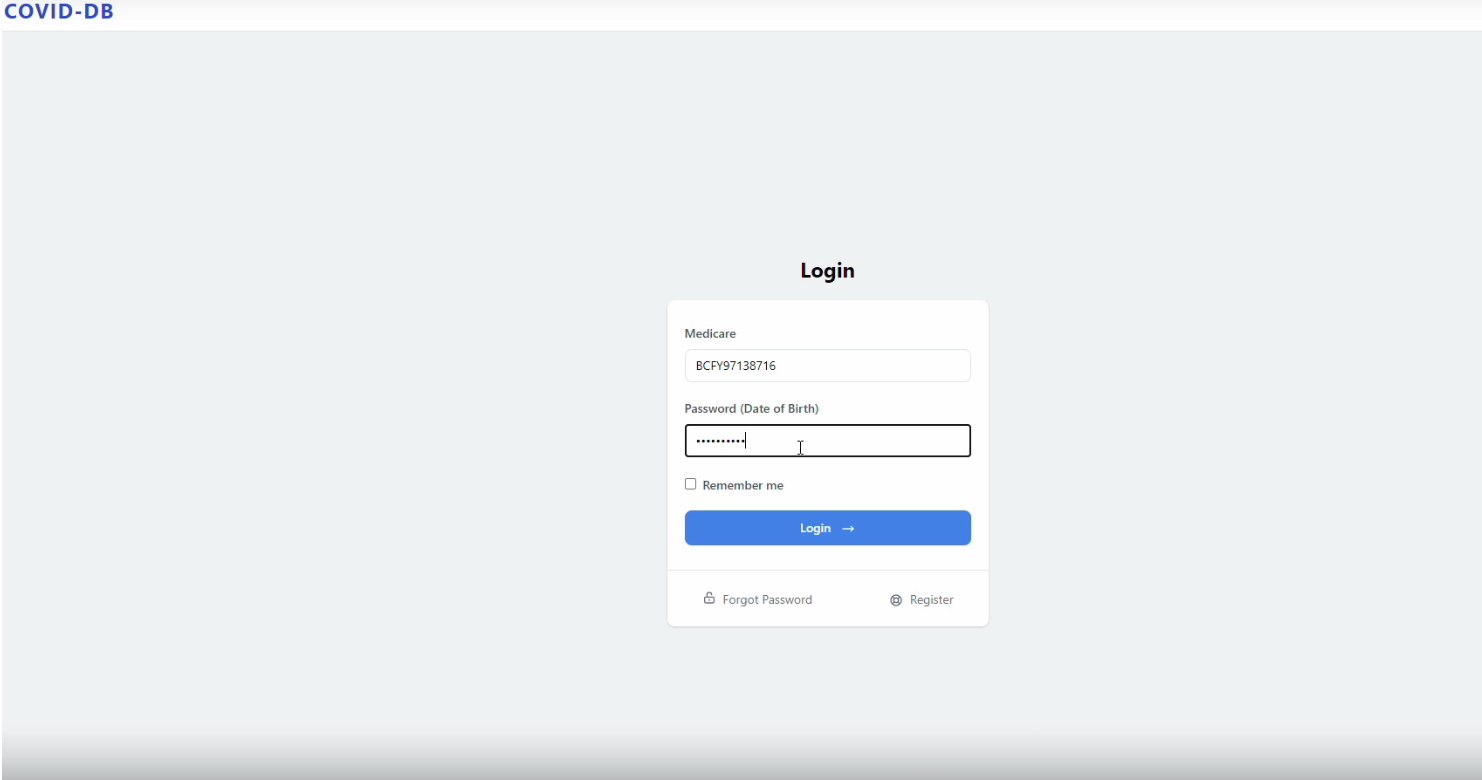
\includegraphics[scale=0.35]{imgs/loginScreen.PNG}}
    \caption{Home Page allows you to login with your medicare and dob}
\end{figure}

